\documentclass[runningheads]{llncs}

%\usepackage{times}
%\usepackage{epsfig}
\usepackage{graphicx}
\usepackage{caption}
%\usepackage{subfigure}
\usepackage{subcaption}
\captionsetup{compatibility=false}
\usepackage{amsmath}
\usepackage{amssymb}
\usepackage{ruler}
\usepackage{color}
\usepackage{booktabs}
\usepackage{mathtools}
%\usepackage{pgfplots}
\usepackage[width=122mm,left=12mm,paperwidth=146mm,height=193mm,top=12mm,paperheight=217mm]{geometry}
%\newtheorem{proposition}{Proposition}
%\newtheorem{lemma}{Lemma}
%\newtheorem{proof}{Proof}
\newcommand{\RR}{\mathbb R}
\newcommand{\NNN}{\mathcal X}
\newcommand{\sumi}{\displaystyle{\sum_{i=1}^n}}
\DeclareMathOperator*{\argmin}{argmin}

% Highlighting
\usepackage{soul}
\usepackage{color}
%\usepackage[usenames,dvipsnames]{xcolor}
\newcommand{\hlc}[2][yellow]{{\sethlcolor{#1}\hl{#2}}}
\newcommand{\RAF}[1]{\hlc[yellow]{(RR:) #1}}
\newcommand{\JZ}[1]{\hlc[pink]{(JZ:) #1}}
\newcommand{\PP}[1]{\hlc[green]{PP: #1}}

\usepackage{tikz}
\usepackage{pgfplots,pgfplotstable}
\usetikzlibrary{pgfplots.groupplots}
\pgfplotsset{grid=major,height=2in, width=\columnwidth}
\tikzset{PolySLEM/.style={mark=*, green}}
\tikzset{GaussSLEM/.style={mark=*, blue}}
\tikzset{ESVM/.style={mark=*, red}}
\tikzset{LinSLEM/.style={mark=*, black}}
\tikzset{VLAD/.style={mark=*, cyan}}
%\tikzset{ussvmne/.style={mark=None, blue, dash pattern=on 4pt off 1pt on 1pt off 1pt}}
%\tikzset{l1svm/.style={mark=*, red, mark options={solid, fill=red!80!black}, solid}}
%\tikzset{l2svm/.style={mark=*, brown!60!black, mark options={solid, fill=brown!80!black}, solid}}


%
\pgfplotsset{compat=newest,legend columns=-1}

\pgfplotstableread{
Criterion   criterion1  criterion2
part1       8           2349
part2       8           452
part3       14          1006
}\first

\pgfplotstableread{
Criterion   criterion1  criterion2
part1       36          10220
part2       36          5891
part3       85          3160
}\second

\pgfplotstableread{
Criterion   criterion1  criterion2
part1       97          25657
part2       97          18306
part3       184         7461
}\third

\begin{document}
% \renewcommand\thelinenumber{\color[rgb]{0.2,0.5,0.8}\normalfont\sffamily\scriptsize\arabic{linenumber}\color[rgb]{0,0,0}}
% \renewcommand\makeLineNumber {\hss\thelinenumber\ \hspace{6mm} \rlap{\hskip\textwidth\ \hspace{6.5mm}\thelinenumber}}
% \linenumbers


\pagestyle{headings}
\mainmatter
\def\ECCV16SubNumber{1390}  % Insert your submission number here

\title{Kernel Square-Loss Exemplar Machines\\ For Image Retrieval: Supplementary Material} % Replace with your title

\titlerunning{ECCV-16 submission ID \ECCV16SubNumber}

\authorrunning{ECCV-16 submission ID \ECCV16SubNumber}

\author{Anonymous ECCV submission}
\institute{Paper ID \ECCV16SubNumber}


\maketitle
%\thispagestyle{empty}

We present here some additional experiments and a discussion of 
different variants of the approach proposed in our submission.



\section{Rotation of Holidays' images}
In our submission, we compare our results to those obtained in the 
original SPoC paper of Babenko and Lempitsky \cite{babenko15}. We were surprised by not 
be able to reproduce their results on the Holidays Benchmark: 
Indeed, \cite{babenko15} reports a mAP of 81.8, but we only managed to obtain a mAP 
of 77.5 (SPoC+PCA+whitening) in our implementation. Upon careful 
examination of their paper, this is due in large part to the fact that 
Babenko and Limpitski manually rotate by 90 degrees some images that are 
not in their natural orientation to compensate for the fact that CNN 
features are not rotation invariant \cite{babenko15,babenko14}. Applying the {\em same} 
rotations to the {\em same} images boosts the performance of our 
implementation of their method to 81.6 mAP (the 0.2 difference is due to a different set of negative images used to learn the PCA matrix and singular values), and the performance of 
our full method (Poly SLEM) to a mAP of 86.1, clearly outperforming \cite{babenko15}. 
Note that, as required by the ECCV submission rules, these results are 
obtained using the {\em exact same} implementation and parameters as in 
our original submission, simply rotating the input images as in \cite{babenko15,babenko14}.
This phenomenon is not observed for the Oxford dataset, where all 
images appear in their "natural" orientation.

These results, shown in Table \ref{tab}, are comparable to the state of the art for the Holidays dataset which, accordingly to \cite{holidaysSOTA}, is 88.1 for all descriptors and 84.7 for global features such as the SPoC+SLEM. To our knowledge, the state of the art for global features in Holidays is 86.0 is \cite{netVLAD}, which again uses the same rotations as [3] and the additional 
experiments reported in this section.

\begin{table*}[!h]
\begin{center}
\caption{Mean average precision results for INRIA Holidays, expressed as percentages. On the left, results for Holidays dataset as presented in our submission. On the right, results for Holidays dataset with images on their natural orientation.}
\setlength{\tabcolsep}{.2em}
%\begin{tabular}{|c|c|c|c|c|c|c|c|}
\small
\begin{tabular}{c@{\hskip 1em}c@{\hskip 1em}c}
\toprule
Dataset & \textbf{Holidays} & \textbf{Holidays (rot)}\\
\midrule
Model, features  & SPoC & SPoC\\
\midrule
Baseline            & 73.1 & 76.4\\
PCA+whitening       & 77.5 & 81.6 \\
E-SVM               & 79.9 & 84.6 \\
Linear SLEM         & 78.3 & 82.3 \\
Gaussian SLEM       & 81.4 & 84.9 \\
Poly SLEM           & \underline{82.0} & \textbf{86.1} \\
Babenko \textit{et al.} \cite{babenko15} & - & 81.8\\
\hline
\label{tab}
\end{tabular}
\end{center}
\end{table*}

\section{Low rank decomposition evaluation}
We present here a more complete evaluation of the low rank decomposition. In this section, we use SPoC features as our base encoding, the polynomial kernel as our kernel function and Holidays dataset (not rotated, for lack of time) images.
As discussed in our submission, a significantly larger pool does not improve results after $15000$ negative examples. Indeed, for a pool of $100000$ negative examples, we obtain mAP 81.5, compared to 82.0 for $14500$ negative examples.
In Figure \ref{full_low}, we take a pool of 100000 negative examples and show their results (mAP and computation time) in green. For this same pool of negatives, we evaluate their low rank decomposition implementation of $r'\in\big\{ \lfloor \frac{10^5}{2^t}\rfloor, \ 0\le t\le 11 \big\}$, and shown their results in black.


We obtain mAP results close to full rank for small values of rank $r'$, at a fraction of the computation time of the full rank. 
As $r'$ increases, performance increases, but the computational cost eventually overcomes that of the full-rank method (around $r'=10000$).

It is not clear today whether it is advantageous to use a lower-rank approximation of the kernel or fewer negative samples.
\begin{figure}[!h]
  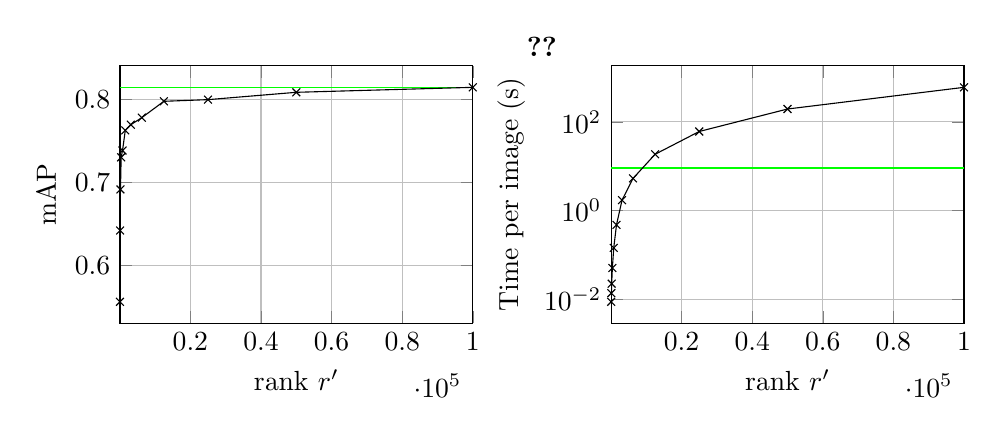
\begin{tikzpicture}
    \begin{groupplot}
      [group style={%
        columns=2,
        rows=1,
        group name=plots,
        xlabels at=edge bottom,
        %y descriptions at=all,
        horizontal sep=5em,        
      },
      % ybar,
      % ymin=0,
      % ymax=27e3,
      enlarge x limits={abs=.5},
      width=0.5\textwidth,
      height=0.4\textwidth,
      % scaled y ticks=base 10:-3,
      % xticklabels from table={\first}{Criterion},
      % x tick label style={rotate=90,anchor=east},
      % xtick=data,
      ]

      \nextgroupplot[xlabel=rank $r'$,
      ylabel=mAP]
      ]
      %% Poly SLEM
      \addplot[green] coordinates {
        (    50,0.815)
        (   100,0.815)
        (   195,0.815)
        (   390,0.815)
        (   781,0.815)
        (  1562,0.815)
        (  3125,0.815)
        (  6250,0.815)
        ( 12500,0.815)
        ( 25000,0.815)
        ( 50000,0.815)
        (100000,0.815)
      };
      \addplot[mark=x, black] coordinates {
        (  50, 0.5560)
         (100, 0.6421)
        ( 195, 0.6917)
        ( 390, 0.73043)
        ( 781, 0.73869)
        ( 1562,0.76307)
        ( 3125,0.76986)
        ( 6250,0.77842)
        (12500,0.79814)
        (25000,0.80014)
        (50000,0.809)
       (100000,0.815)
      };
      
      \nextgroupplot[
      ymode=log,
      xlabel=rank $r'$,
      ylabel=Time per image (s),
      legend to name=grouplegend,
      legend style={legend columns=-1},
      % legend style={at={(0.465,-0.45)},
      % anchor=north,legend columns=-1},
      ]%
      %% Poly SLEM
      \addplot[green] coordinates {
        (    50,9.1)
        (   100,9.1)
        (   195,9.1)
        (   390,9.1)
        (   781,9.1)
        (  1562,9.1)
        (  3125,9.1)
        (  6250,9.1)
        ( 12500,9.1)
        ( 25000,9.1)
        ( 50000,9.1)
        (100000,9.1)
      };
      \addlegendentry{Full rank}
      \addplot[mark=x, black] coordinates {
        (  50, 0.0088)
         (100, 0.0138)
        ( 195, 0.0225)
        ( 390, 0.0508)
        ( 781, 0.1446)
        (1562, 0.4762)
        (3125, 1.717)
        (6250, 5.317)
        (12500,18.56)
        (25000,60.54)
        (50000,194.2)
       (100000,598)
      };
      \addlegendentry{Low rank}
      
    \end{groupplot}

    \node at (plots c1r1.north east) [anchor=south, xshift=2.5em] {\ref{grouplegend}};
    %\draw (plots c2r1.north west) circle (3pt) node {North west};

  \end{tikzpicture}
  \caption{Results for INRIA Holidays, using SPoC as base features and PolySLEM. In green, we report full rank results for $n=100000$. In black, we report a low rank approximation for $n=100000$ and rank $r'$ varying axis $x$. On the left, mAP results for each model. On the right, running time per positive image.}
  \label{full_low}
\end{figure}



%% Local Variables:
%% TeX-master: "main_eccv"
%% End:
%\begin{figure}[!h]
\centering
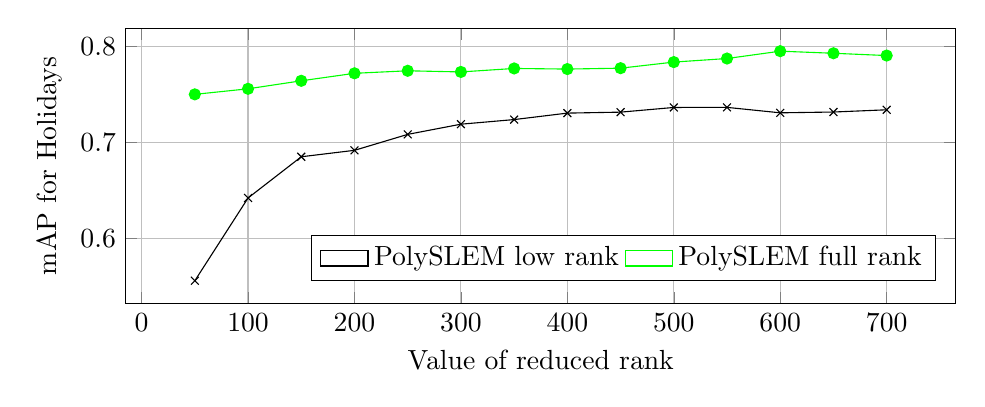
\begin{tikzpicture}
	\begin{axis}[
		xlabel=Value of reduced rank,
		ylabel=mAP for Holidays,
		legend style={
			area legend,
			at={(0.6,0.25)},
			anchor=north,
			legend columns=-1}]
%%Poly SLEM
    \addplot[mark=x, black] coordinates{
         ( 50, 0.5560)
         (100, 0.6421)
         (150, 0.6850)
         (200, 0.6917)
         (250, 0.7083)
         (300, 0.7189)
         (350, 0.7237)
         (400, 0.73043)
         (450, 0.73143)
         (500, 0.73631)
         (550, 0.73639)
         (600, 0.73073)
         (650, 0.73156)
         (700, 0.73388)
    };
    \addlegendentry{PolySLEM low rank}
    \addplot[mark=*, green] coordinates{
        (  50, 0.74994)
        ( 100, 0.75572)
        ( 150, 0.76405)
        ( 200, 0.77184)
       (  250, 0.77447)
         (300, 0.77327)
         (350, 0.77689)
         (400, 0.77626)
         (450, 0.77718)
         (500, 0.78352)
         (550, 0.78723)
         (600, 0.79487)
         (650, 0.79270)
         (700, 0.79032)
    };
    \addlegendentry{PolySLEM full rank}
	\end{axis}
\end{tikzpicture}
\caption{mAP for Holidays using SPoC features. We perform a low-rank decomposition of a $100000\times 100000$ kernel matrix for the low rank curve, whereas we use a full rank decomposition with }
\end{figure}


%We then compare the low rank results for rank equals $r'$ to a full rank decomposition of a pool of $r'$ negative examples, for very small values of $r'$. What we observe is that a full rank decomposition obtain better retrieval results, even 

\section{More large scale retrieval results}
In our submission, we compare our large scale results to those obtained in \cite{ZePe15} with recursive ESVM (RESVM-2) in the Oxford 5k benchmark using VLAD-64 as base features. 
We did not had at the time finished the same experiment for the Holidays dataset, in part due to our results not being superior to those presented in \cite{ZePe15}. 
We present them in Figure \ref{vlad:holidays}, for multiple kernel SLEMs, ESVM and RESVM-2 presented by \cite{ZePe15}. 
\begin{figure}[!h]
\centering
\begin{tikzpicture}
	\begin{semilogxaxis}[
		xlabel=Number of distractors,
		ylabel=mAP,
		legend to name=vladholidays,
        legend style={legend columns=-1}]
		%legend = south west]
%%Poly SLEM
    \addplot[PolySLEM] coordinates{
        (   0, 0.77958)
        (1000, 0.77676)
        (3000, 0.77018)
        (6000, 0.76609)
       (10000, 0.76408)
       (30000, 0.75422)
       (60000, 0.74716)
      (100000, 0.73867)
      (300000, 0.71629)
      (600000, 0.69856)
    };
    \addlegendentry{PolySLEM}
	\addplot[ESVM] coordinates{
        (   0, 0.78269)
        (1000, 0.78112)
        (3000, 0.77622)
        (6000, 0.77255)
       (10000, 0.77002)
       (30000, 0.75942)
       (60000, 0.75050)
      (100000, 0.74132)
      (300000, 0.72561)
      (600000, 0.70604)
    };	
    \addlegendentry{RESVM-2}
    \addplot[GaussSLEM] coordinates{
        (   0, 0.77917)
        (1000, 0.77907)
        (3000, 0.76933)
        (6000, 0.76528)
       (10000, 0.76327)
       (30000, 0.75273)
       (60000, 0.74686)
      (100000, 0.73825)
      (300000, 0.72029)
      (600000, 0.7)
    };
    \addlegendentry{GaussSLEM}
    \addplot[LinSLEM] coordinates{
        (   0, 0.77966)
        (1000, 0.76369)
        (3000, 0.75864)
        (6000, 0.75391)
       (10000, 0.74994)
       (30000, 0.73902)
       (60000, 0.73228)
      (100000, 0.72664)
      (300000, 0.71048)
      (600000, 0.69126)
    };
    \addlegendentry{LinSLEM}
    \addplot[mark=o, red] coordinates{
        (   0, 0.77778)
        (1000, 0.77372)
        (3000, 0.76578)
        (6000, 0.76221)
       (10000, 0.75956)
       (30000, 0.74938)
       (60000, 0.7415)
      (100000, 0.73256)
      (300000, 0.71456)
      (600000, 0.69278)
    };
    \addlegendentry{ESVM-1}
	\end{semilogxaxis}
	\node at (plots c1r1.north east) [anchor=south, xshift=2.8em] {\ref{vladholidays}};
\end{tikzpicture}
\caption{mAP for INRIA Holidays using SPoC as base features and PolySLEM, full rank and low rank decompositions.}
\label{vlad:holidays}
\end{figure}





\section{Recursive square loss exemplar machine?} \label{RSLEM}
One interesting process proposed in \cite{ZePe15} is the recursive exemplar SVM encoding (or RESVM). The proposed idea is to implement the encoding pipeline $k$ times, $k>0$, taking the output of the $(k-1)$-th ESVM pipeline as input of the $k$-th ESVM pipeline. Here, we consider the base features as the output of the of the 0-th ESVM pipeline. 
Indeed, if write $\omega^\star$ as a function of the positive exemplar $x_0$ and the pool of negative examples $\NNN=\{x_1,x_2,...,x_n\}$\footnote{In our submission, we treated the pool of negatives as a matrix $X$. Exceptionally in this section, we treat the pool as a set in order to facilitate our notation}, \emph{i.e.}, 
\begin{equation}
\omega^\star(x_0, \NNN) = \argmin_{\omega\in\RR^d} \left(\theta \ l(1, \omega^Tx_0+\nu^\star) +\dfrac{1}{n}\sum_{x_i\in\NNN}l(1, \omega^Tx_i+\nu^\star)+\dfrac{\lambda}{2}\|\omega\|^2\right),
\end{equation}
and we denote the baseline encodings as $\omega^{(0)}=x_0$ and $\NNN^{(0)}=\NNN$,
the $k$-th recursion of ESVM is given by $\omega^{(k)}(x_0, \NNN) = \omega^\star (\omega^{(k-1)}, \NNN^{(k-1)})$, where $\NNN^{(k)} = \{\omega^\star(z, \NNN^{(k-1)}\setminus \{z\}), \ z\in\NNN^{(k-1)} \}$.
Note that the application of the $k$-th pipeline depends on the application of the $(k-1)$-th pipeline on the negative examples. In \cite{ZePe15}, this means taking the pool of negatives equals to $\NNN \setminus \{x_i\}$ for each negative example $x_i$. However, for SLEM, it means recalculating the matrix $A$ for each different pool of negative examples. This makes a recursive SLEM much more time costly than a regular SLEM, negating the computational advantages of 
our approach. Thus, we have not implemented recursive SLEM. One could 
also imagine keeping the positive example among the negative ones, which 
would avoid recomputing A at each iteration, but does not make much sense. Indeed, it would mean solving a classification problem where the only positive example is also a negative example.



\begin{equation}
    x_0\in \RR^d
\end{equation}
%The other alternative is to not exclude the positive example of the pool of negative, \emph{i.e.}, 
%$\NNN^{(k)} = \{\omega^\star(z, \NNN^{(k-1)}), \ z\in\NNN^{(k-1)} \}$. This avoids the recalculation of matrix $A$, but it means we solve a classification problem where the only positive example is also a negative example for each element in $\NNN$. As a result, in our experiments with recursive SLEM, we obtain a mAP 0.5 percentage points inferior to the regular SLEM results. These results were obtained in Holidays dataset, for Gaussian, linear kernels and $k=2$ recursive encodings.

\bibliographystyle{ieee} 
\bibliography{sup,jz}
\end{document}


	
%% Local Variables:
%% TeX-master: "suppmat"
%% End:
